More details on electron reconstruction can be found in Ref.~\cite{ElectronLegacy}. 

Electron candidates are preselected using loose cuts on track-cluster matching observables, so as to preserve the highest possible efficiency while rejecting part of the QCD background. To be considered for the analysis, electrons are required to have a
transverse momentum $p^e_T >$ 7 GeV, a reconstructed $|\eta^e| <$ 2.5, and to satisfy a loose primary vertex 
constraint defined as $d_{xy} < 0.5$ cm and $d_z < 1$ cm.
Such electrons are called {\bf loose electrons}.

The data-MC discrepancy is corrected using scale factors as is done for the electron selection with data efficiencies measured using the same tag-and-probe technique outlined later (see Section~\ref{sec:eleEffMeas}). 
These studies for reconstructions are carried out by the EGM POG and the results are only summarised here.

The electron reconstruction scale factors are shown Fig.~\ref{fig:ele_rec_scale_factors} and are applied as a function of the super cluster $\eta$ and electron $\pt$.

\begin{figure}[!htb]
\vspace*{0.3cm}
\begin{center}
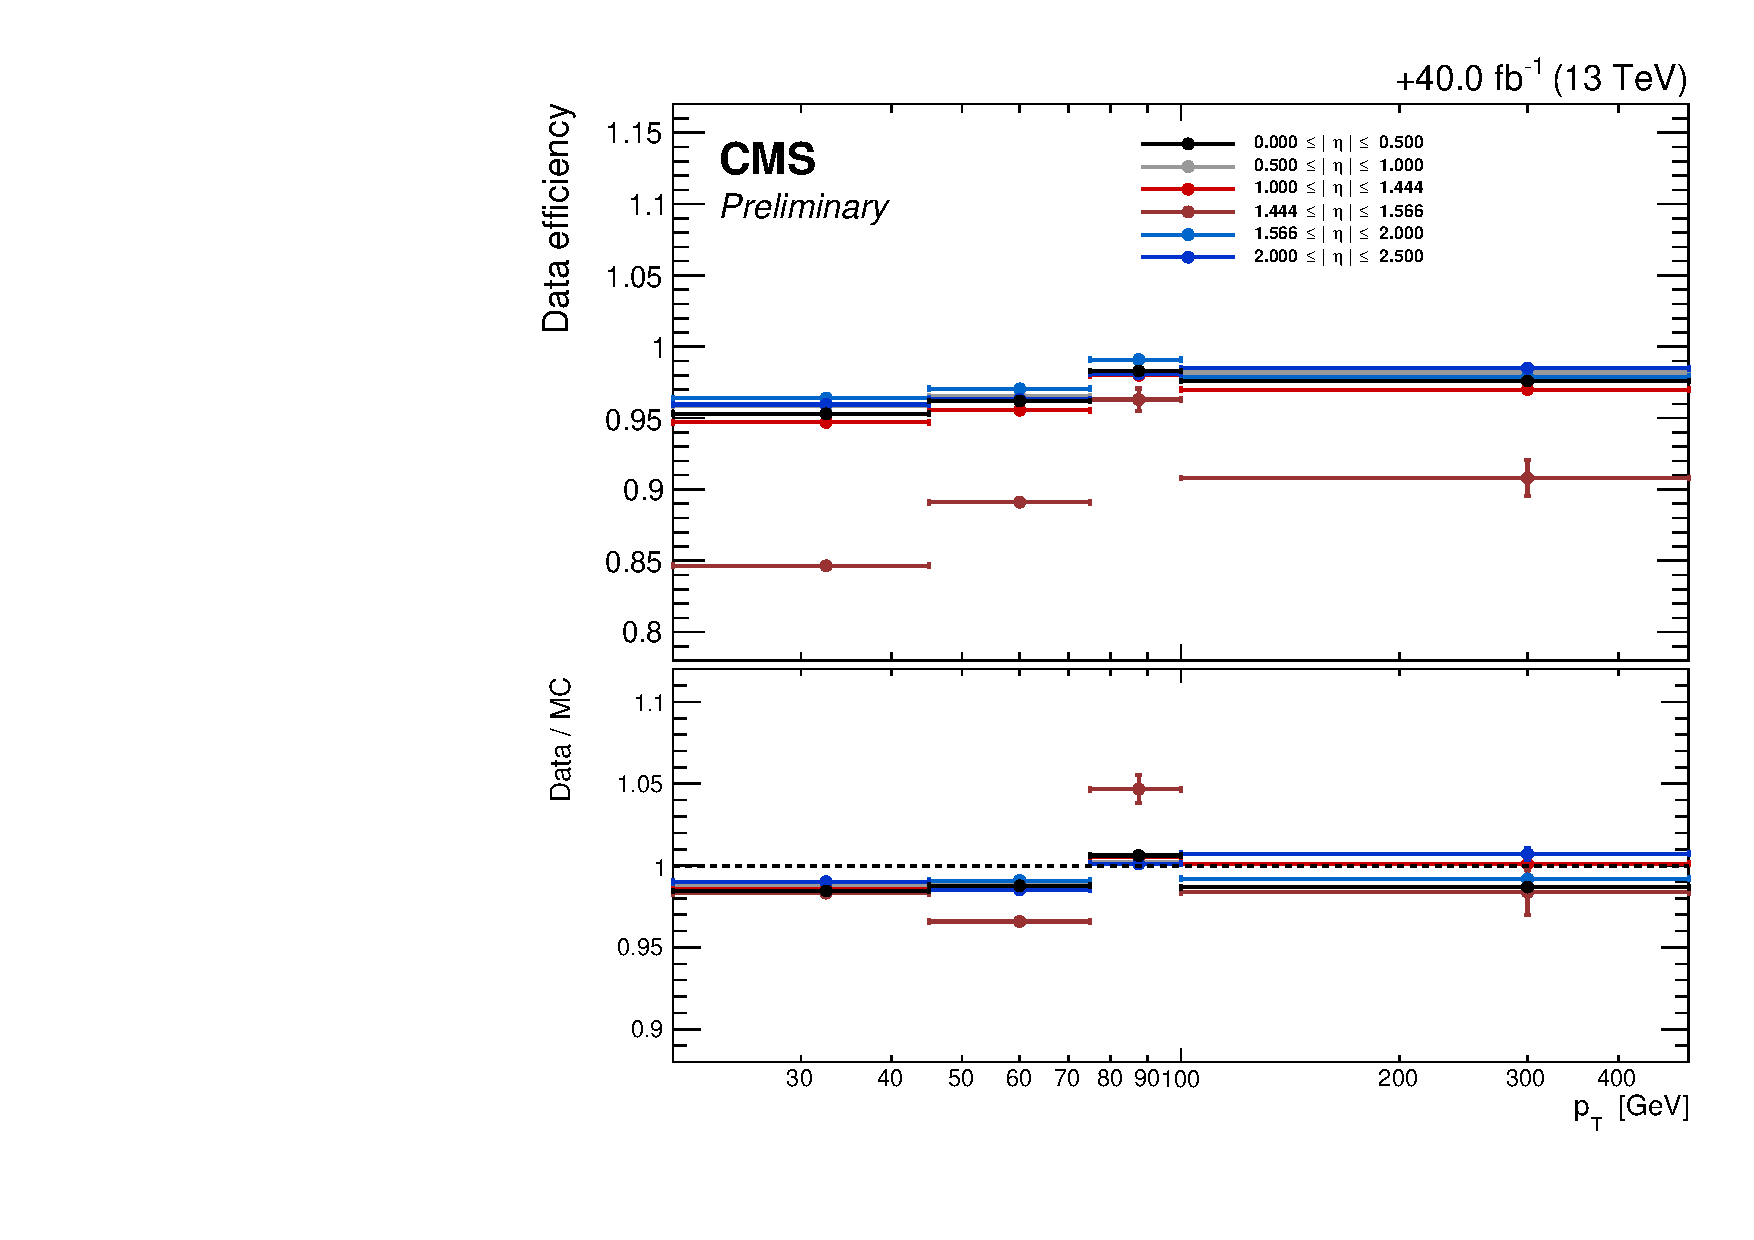
\includegraphics[width=0.4\textwidth]{Figures/Electrons/ErecoPt}
\includegraphics[page=2, width=0.4\textwidth]{Figures/Electrons/ErecoEta}\\
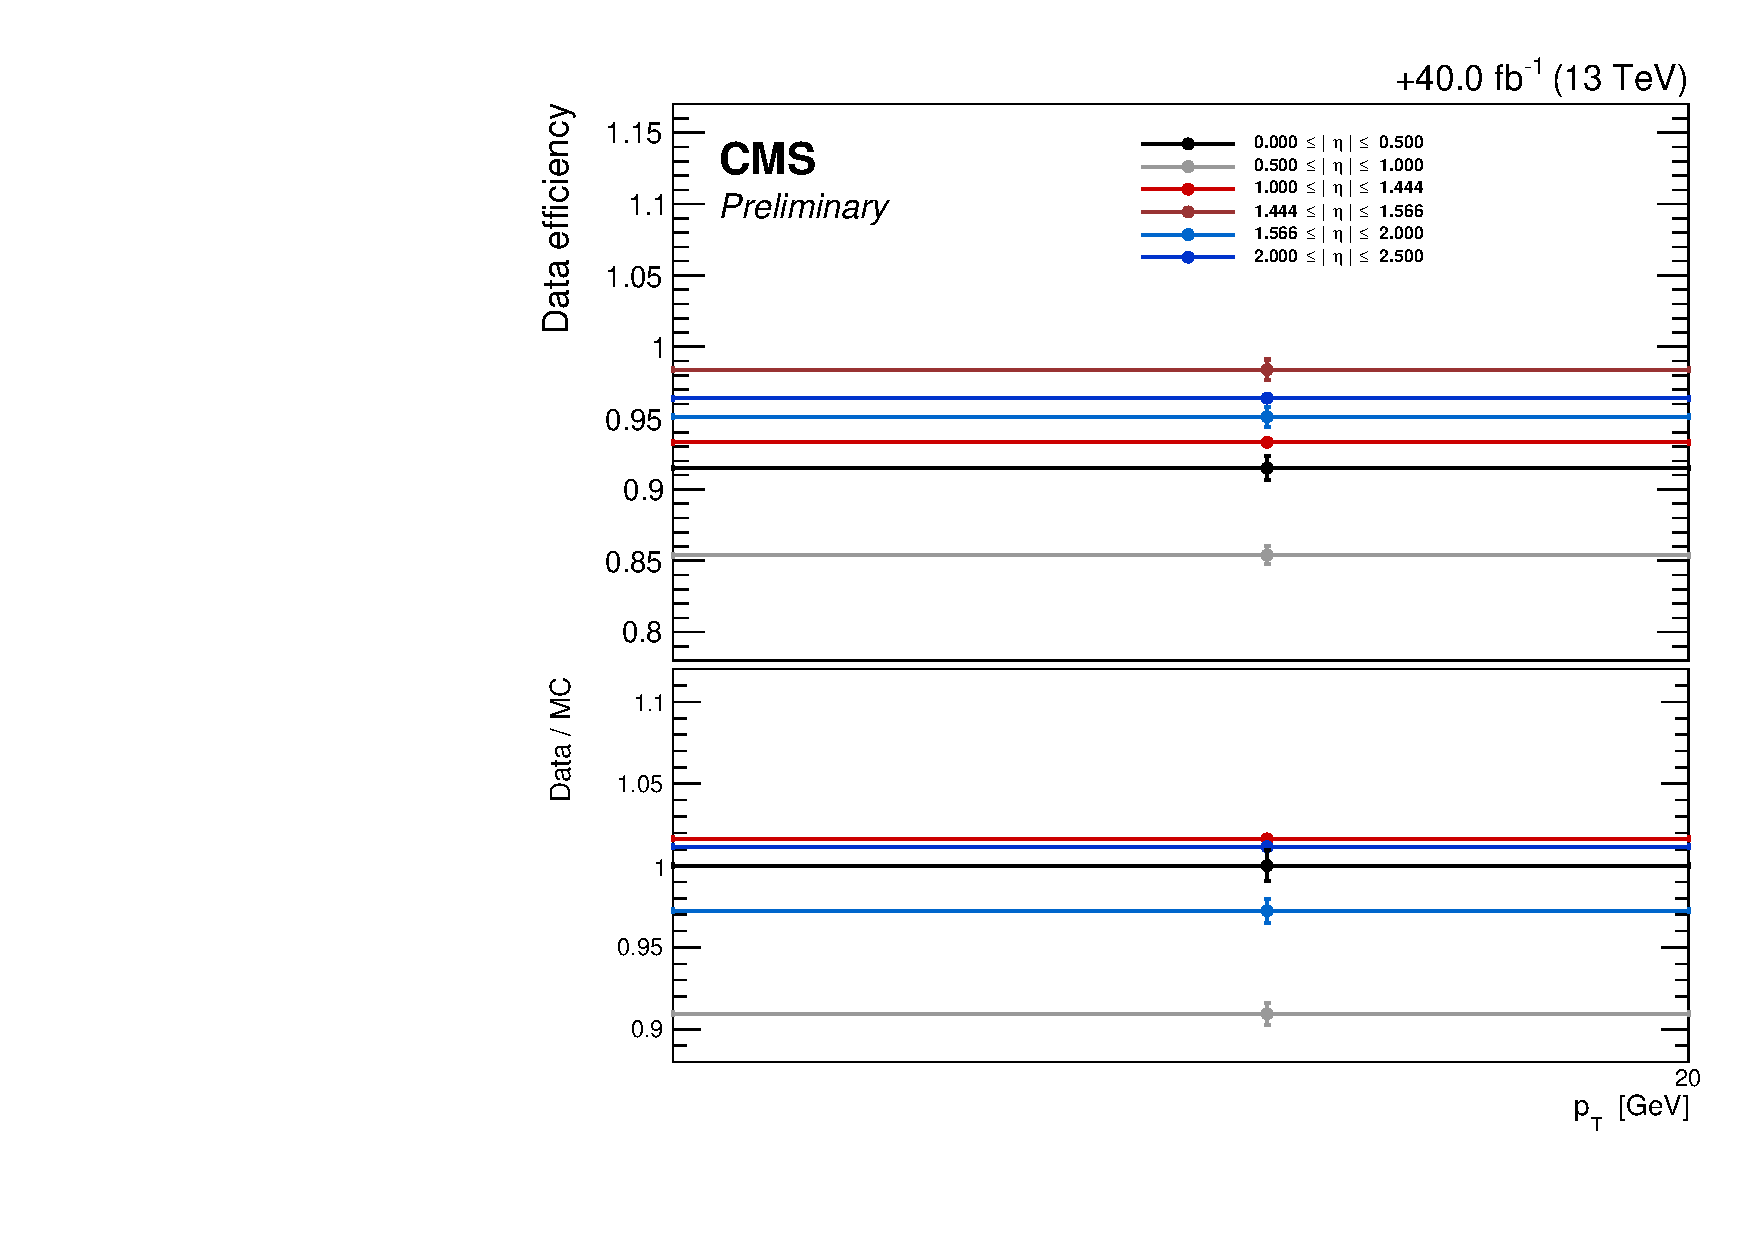
\includegraphics[width=0.4\textwidth]{Figures/Electrons/ErecoPt_lowPt}
%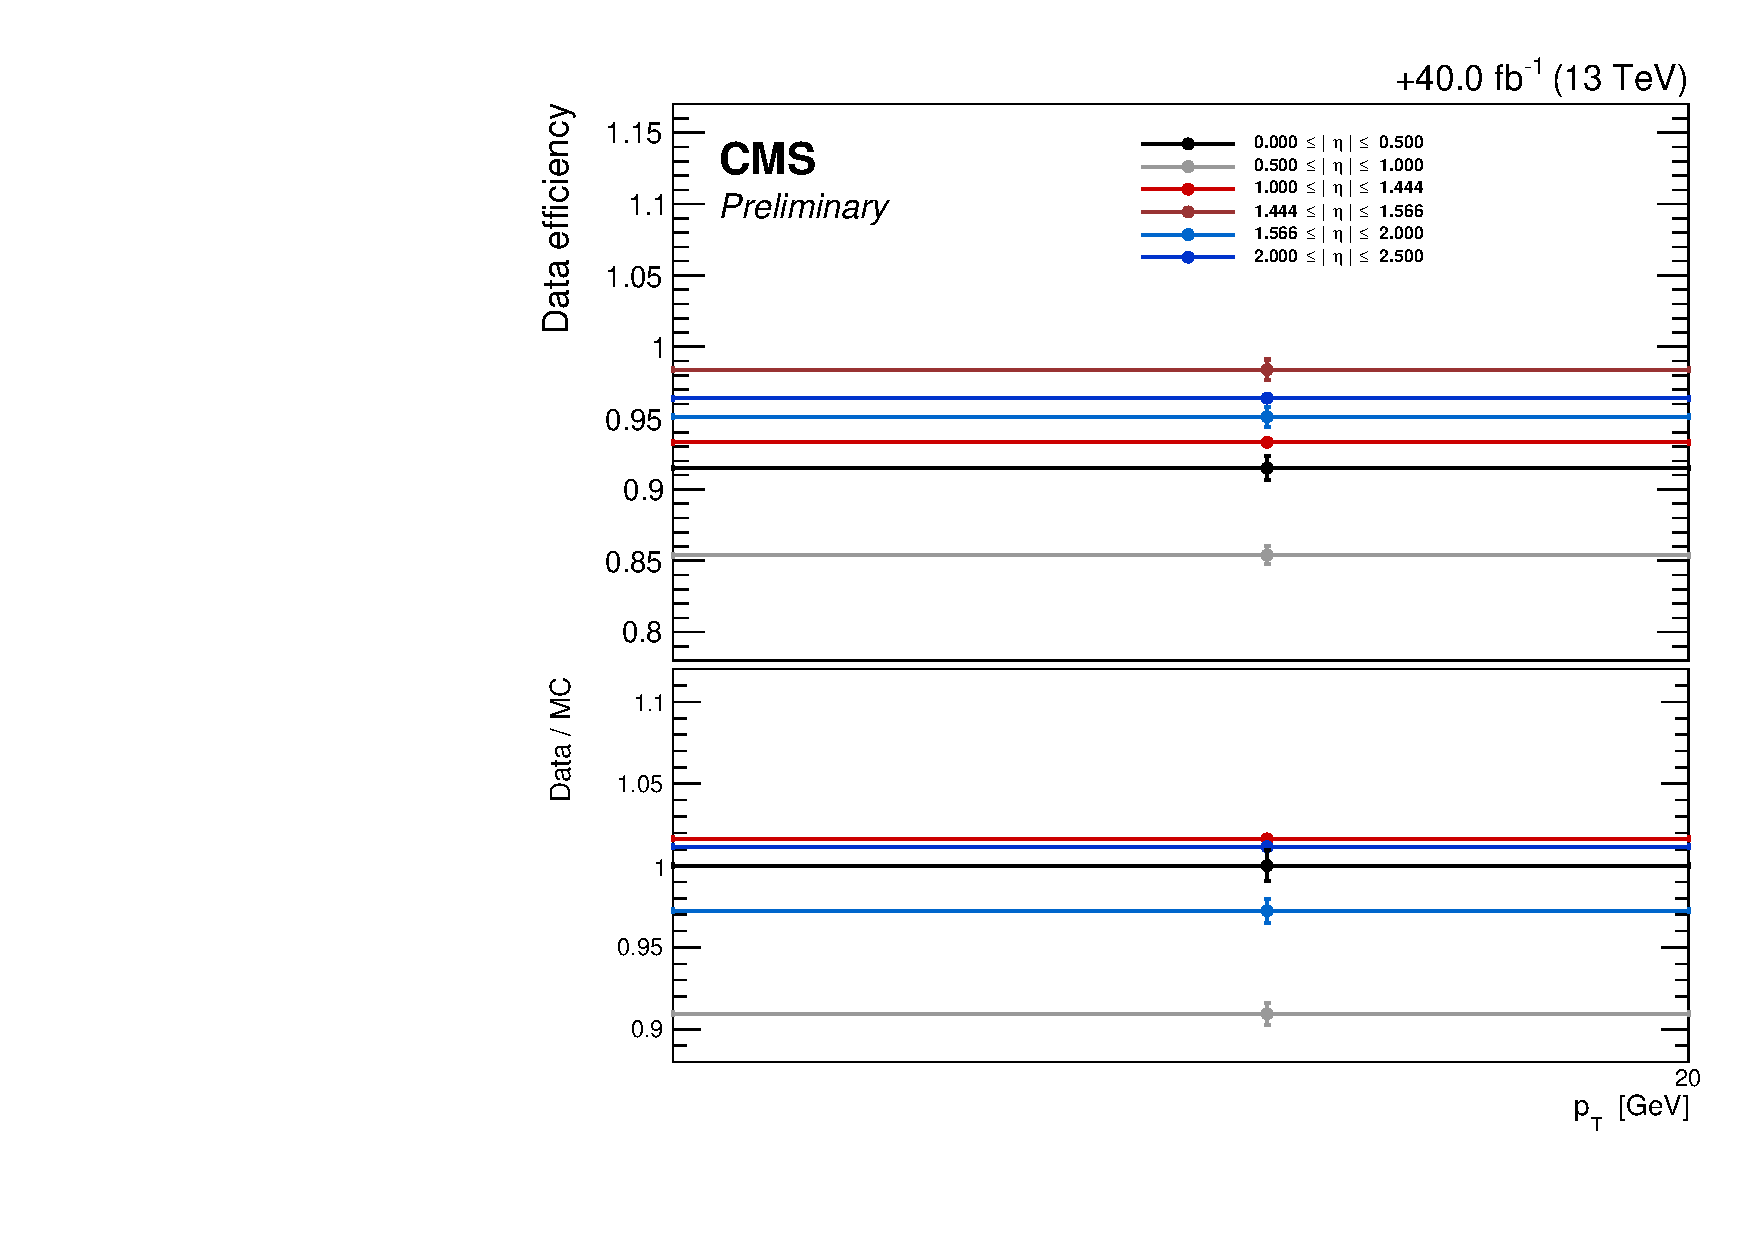
\includegraphics[width=0.4\textwidth]{Figures/Electrons/ErecoEta_lowPt}
\end{center}
\caption{Electron reconstruction efficiencies efficiency in data versus $p_T$ (left) and $\eta$ (right) for electrons with $\pt > 20 \GeV$ (top) and $\pt < 20 \GeV$ (bottom) with corresponding data/MC scale factors as provided by the EGM POG. Errors are statistical only. }
\label{fig:ele_rec_scale_factors}
\end{figure}


